\documentclass[tikz,border=1cm]{standalone}

\usepackage{tikz}
\usetikzlibrary{%
    decorations.pathreplacing,%
    decorations.pathmorphing%
}

%%%%%%%%%%%%Todo está en 2D porque no entiendo 3D   :c
\begin{document}


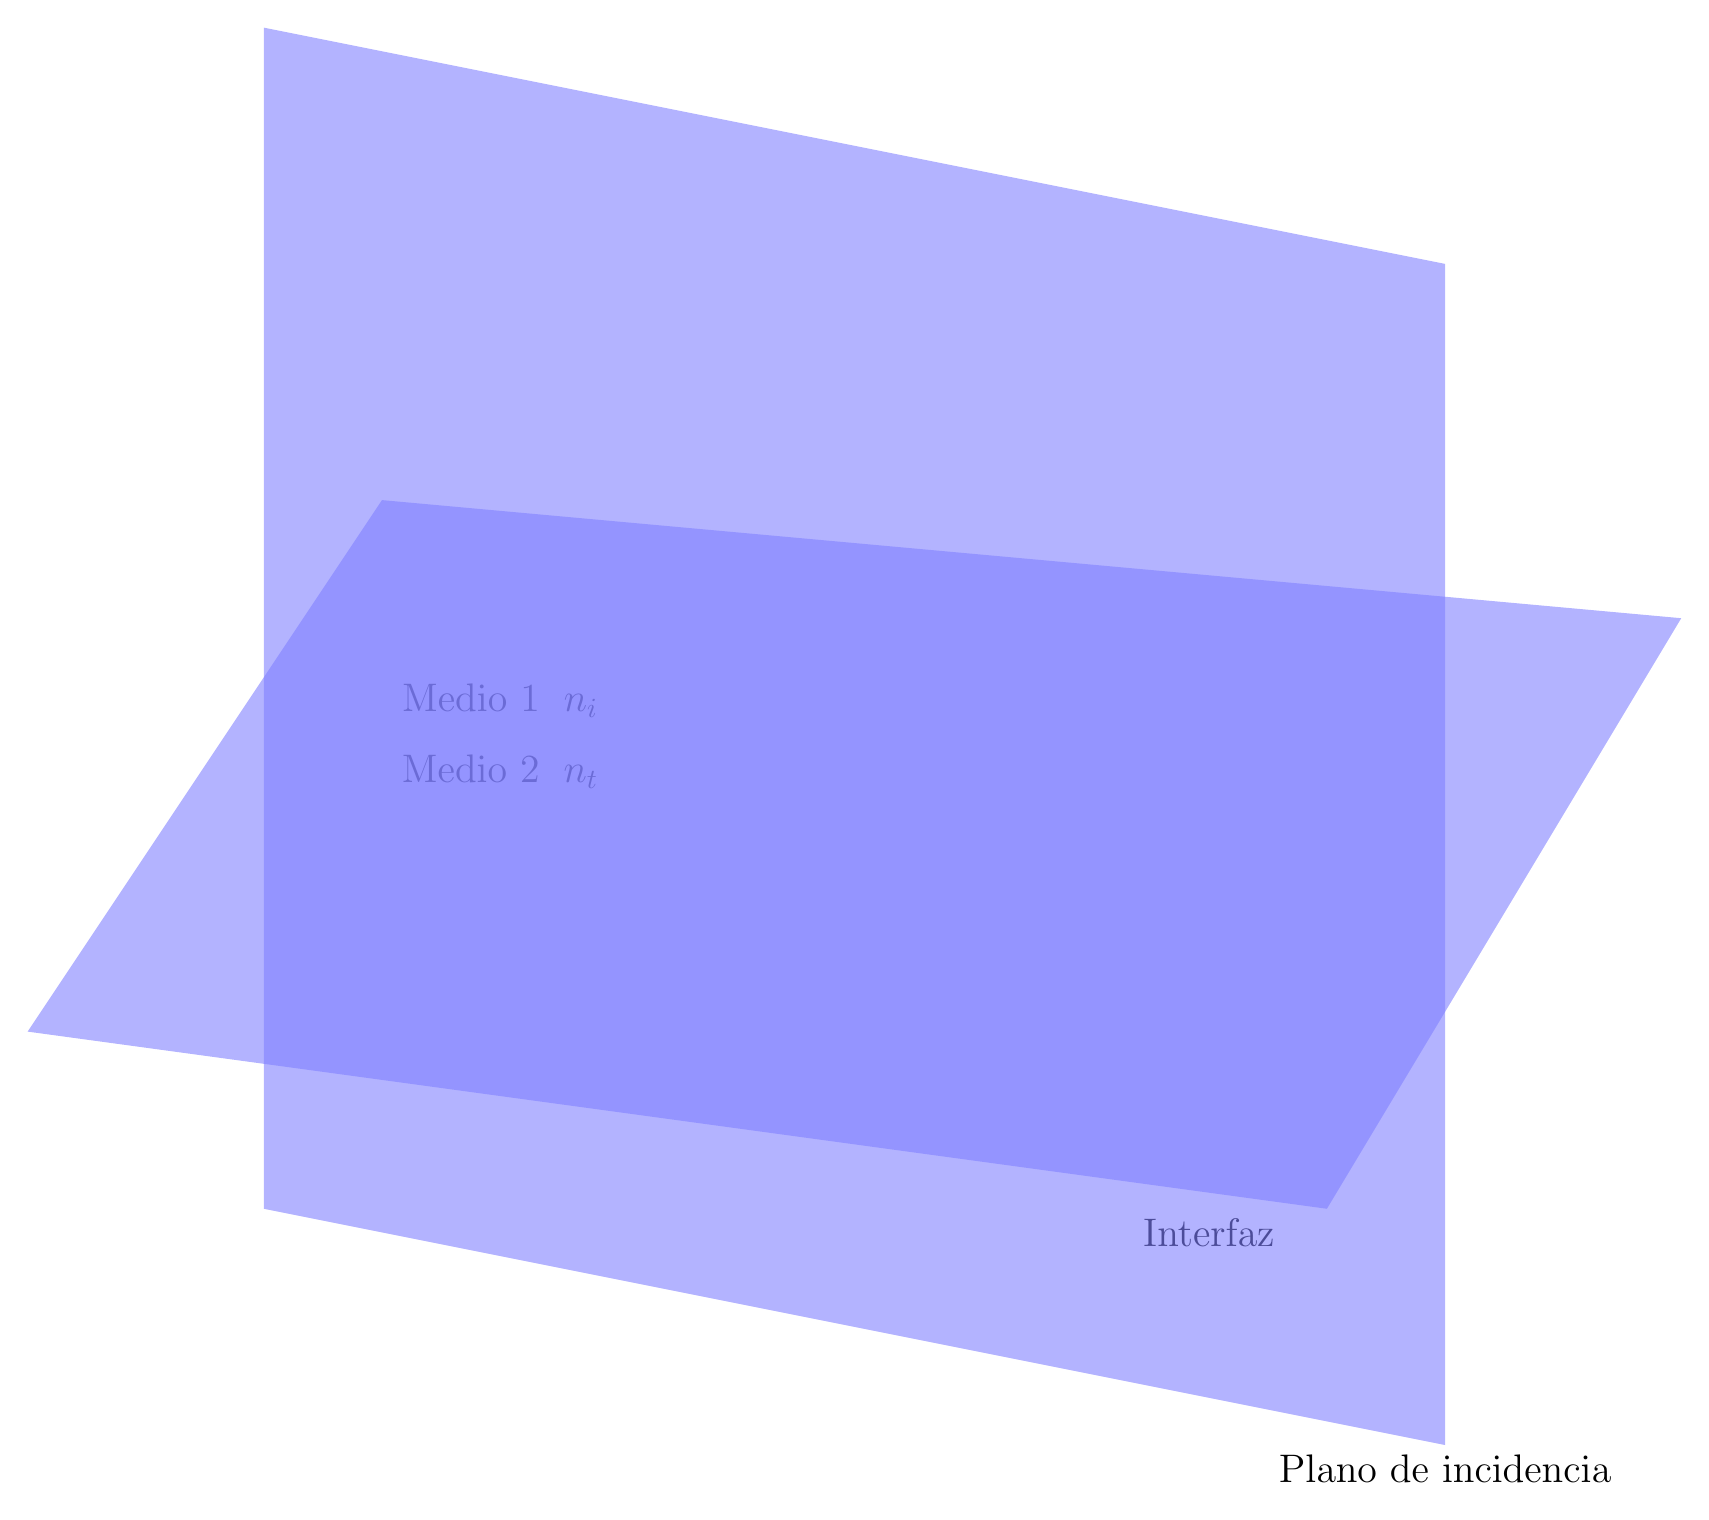
\begin{tikzpicture}[scale =1.5]


\path (3,-4)node[color = black,below]{\Large Interfaz};
\path (5,-6)node[color = black,below]{\Large Plano de incidencia};
\node at (-3,.3) { \Large Medio 1 $\; n_i$}; 
\node at (-3,-.3) {\Large Medio 2 $\; n_t$};
\fill[blue!50, opacity =.6] (-7,-2.5) -- (-4,2) -- (7,1) -- (4,-4) -- (-7,-2.5);  %interfaz
\fill[blue!50, opacity =.6] (-5,-4) -- (-5,6) -- (5,4) -- (5,-6) --  (-5,-4);   %plano de incidencia



\end{tikzpicture}


\end{document}